%**************************************%
%* Generated from MathBook XML source *%
%*    on 2018-09-06T09:07:06-05:00    *%
%*                                    *%
%*   http://mathbook.pugetsound.edu   *%
%*                                    *%
%**************************************%
\documentclass[10pt,]{book}
%% Custom Preamble Entries, early (use latex.preamble.early)
%% Inline math delimiters, \(, \), need to be robust
%% 2016-01-31:  latexrelease.sty  supersedes  fixltx2e.sty
%% If  latexrelease.sty  exists, bugfix is in kernel
%% If not, bugfix is in  fixltx2e.sty
%% See:  https://tug.org/TUGboat/tb36-3/tb114ltnews22.pdf
%% and read "Fewer fragile commands" in distribution's  latexchanges.pdf
\IfFileExists{latexrelease.sty}{}{\usepackage{fixltx2e}}
%% Text height identically 9 inches, text width varies on point size
%% See Bringhurst 2.1.1 on measure for recommendations
%% 75 characters per line (count spaces, punctuation) is target
%% which is the upper limit of Bringhurst's recommendations
%% Load geometry package to allow page margin adjustments
\usepackage{geometry}
\geometry{letterpaper,total={340pt,9.0in}}
%% Custom Page Layout Adjustments (use latex.geometry)
%% This LaTeX file may be compiled with pdflatex, xelatex, or lualatex
%% The following provides engine-specific capabilities
%% Generally, xelatex and lualatex will do better languages other than US English
%% You can pick from the conditional if you will only ever use one engine
\usepackage{ifthen}
\usepackage{ifxetex,ifluatex}
\ifthenelse{\boolean{xetex} \or \boolean{luatex}}{%
%% begin: xelatex and lualatex-specific configuration
%% fontspec package will make Latin Modern (lmodern) the default font
\ifxetex\usepackage{xltxtra}\fi
\usepackage{fontspec}
%% realscripts is the only part of xltxtra relevant to lualatex 
\ifluatex\usepackage{realscripts}\fi
%% 
%% Extensive support for other languages
\usepackage{polyglossia}
\setdefaultlanguage{english}
%% Magyar (Hungarian)
\setotherlanguage{magyar}
%% Spanish
\setotherlanguage{spanish}
%% Vietnamese
\setotherlanguage{vietnamese}
%% end: xelatex and lualatex-specific configuration
}{%
%% begin: pdflatex-specific configuration
%% translate common Unicode to their LaTeX equivalents
%% Also, fontenc with T1 makes CM-Super the default font
%% (\input{ix-utf8enc.dfu} from the "inputenx" package is possible addition (broken?)
\usepackage[T1]{fontenc}
\usepackage[utf8]{inputenc}
%% end: pdflatex-specific configuration
}
%% Monospace font: Inconsolata (zi4)
%% Sponsored by TUG: http://levien.com/type/myfonts/inconsolata.html
%% See package documentation for excellent instructions
%% One caveat, seem to need full file name to locate OTF files
%% Loads the "upquote" package as needed, so we don't have to
%% Upright quotes might come from the  textcomp  package, which we also use
%% We employ the shapely \ell to match Google Font version
%% pdflatex: "varqu" option produces best upright quotes
%% xelatex,lualatex: add StylisticSet 1 for shapely \ell
%% xelatex,lualatex: add StylisticSet 2 for plain zero
%% xelatex,lualatex: we add StylisticSet 3 for upright quotes
%% 
\ifthenelse{\boolean{xetex} \or \boolean{luatex}}{%
%% begin: xelatex and lualatex-specific monospace font
\usepackage{zi4}
\setmonofont[BoldFont=Inconsolatazi4-Bold.otf,StylisticSet={1,3}]{Inconsolatazi4-Regular.otf}
%% end: xelatex and lualatex-specific monospace font
}{%
%% begin: pdflatex-specific monospace font
\usepackage[varqu]{zi4}
%% end: pdflatex-specific monospace font
}
%% Symbols, align environment, bracket-matrix
\usepackage{amsmath}
\usepackage{amssymb}
%% allow more columns to a matrix
%% can make this even bigger by overriding with  latex.preamble.late  processing option
\setcounter{MaxMatrixCols}{30}
%%
%% Color support, xcolor package
%% Always loaded.  Used for:
%% mdframed boxes, add/delete text, author tools
\PassOptionsToPackage{usenames,dvipsnames,svgnames,table}{xcolor}
\usepackage{xcolor}
%%
%% Semantic Macros
%% To preserve meaning in a LaTeX file
%% Only defined here if required in this document
%% Subdivision Numbering, Chapters, Sections, Subsections, etc
%% Subdivision numbers may be turned off at some level ("depth")
%% A section *always* has depth 1, contrary to us counting from the document root
%% The latex default is 3.  If a larger number is present here, then
%% removing this command may make some cross-references ambiguous
%% The precursor variable $numbering-maxlevel is checked for consistency in the common XSL file
\setcounter{secnumdepth}{3}
%% Environments with amsthm package
%% Theorem-like environments in "plain" style, with or without proof
\usepackage{amsthm}
\theoremstyle{plain}
%% Numbering for Theorems, Conjectures, Examples, Figures, etc
%% Controlled by  numbering.theorems.level  processing parameter
%% Always need a theorem environment to set base numbering scheme
%% even if document has no theorems (but has other environments)
\newtheorem{theorem}{Theorem}[section]
%% Only variants actually used in document appear here
%% Style is like a theorem, and for statements without proofs
%% Numbering: all theorem-like numbered consecutively
%% i.e. Corollary 4.3 follows Theorem 4.2
\newtheorem{corollary}[theorem]{Corollary}
%% Definition-like environments, normal text
%% Numbering is in sync with theorems, etc
\theoremstyle{definition}
\newtheorem{definition}[theorem]{Definition}
%% Example-like environments, normal text
%% Numbering is in sync with theorems, etc
\theoremstyle{definition}
\newtheorem{example}[theorem]{Example}
%% Miscellaneous environments, normal text
%% Numbering for inline exercises and lists is in sync with theorems, etc
\theoremstyle{definition}
\newtheorem{exercise}[theorem]{Exercise}
%% Localize LaTeX supplied names (possibly none)
\renewcommand*{\proofname}{Proof}
\renewcommand*{\chaptername}{Chapter}
%% Equation Numbering
%% Controlled by  numbering.equations.level  processing parameter
\numberwithin{equation}{section}
%% For improved tables
\usepackage{array}
%% Some extra height on each row is desirable, especially with horizontal rules
%% Increment determined experimentally
\setlength{\extrarowheight}{0.2ex}
%% Define variable thickness horizontal rules, full and partial
%% Thicknesses are 0.03, 0.05, 0.08 in the  booktabs  package
\makeatletter
\newcommand{\hrulethin}  {\noalign{\hrule height 0.04em}}
\newcommand{\hrulemedium}{\noalign{\hrule height 0.07em}}
\newcommand{\hrulethick} {\noalign{\hrule height 0.11em}}
% TeX imported from a WeBWorK server might use booktabs rule commands
% Replace/delete these three approximations if booktabs is loaded
\newcommand{\toprule}{\hrulethick}
\newcommand{\midrule}{\hrulemedium}
\newcommand{\bottomrule}{\hrulethick}
%% We preserve a copy of the \setlength package before other
%% packages (extpfeil) get a chance to load packages that redefine it
\let\oldsetlength\setlength
\newlength{\Oldarrayrulewidth}
\newcommand{\crulethin}[1]%
{\noalign{\global\oldsetlength{\Oldarrayrulewidth}{\arrayrulewidth}}%
\noalign{\global\oldsetlength{\arrayrulewidth}{0.04em}}\cline{#1}%
\noalign{\global\oldsetlength{\arrayrulewidth}{\Oldarrayrulewidth}}}%
\newcommand{\crulemedium}[1]%
{\noalign{\global\oldsetlength{\Oldarrayrulewidth}{\arrayrulewidth}}%
\noalign{\global\oldsetlength{\arrayrulewidth}{0.07em}}\cline{#1}%
\noalign{\global\oldsetlength{\arrayrulewidth}{\Oldarrayrulewidth}}}
\newcommand{\crulethick}[1]%
{\noalign{\global\oldsetlength{\Oldarrayrulewidth}{\arrayrulewidth}}%
\noalign{\global\oldsetlength{\arrayrulewidth}{0.11em}}\cline{#1}%
\noalign{\global\oldsetlength{\arrayrulewidth}{\Oldarrayrulewidth}}}
%% Single letter column specifiers defined via array package
\newcolumntype{A}{!{\vrule width 0.04em}}
\newcolumntype{B}{!{\vrule width 0.07em}}
\newcolumntype{C}{!{\vrule width 0.11em}}
\makeatother
%% Figures, Tables, Listings, Floats
%% The [H]ere option of the float package fixes floats in-place,
%% in deference to web usage, where floats are totally irrelevant
%% We re/define the figure, table and listing environments, if used
%%   1) New mbxfigure and/or mbxtable environments are defined with float package
%%   2) Standard LaTeX environments redefined to use new environments
%%   3) Standard LaTeX environments redefined to step theorem counter
%%   4) Counter for new environments is set to the theorem counter before caption
%% You can remove all this figure/table setup, to restore standard LaTeX behavior
%% HOWEVER, numbering of figures/tables AND theorems/examples/remarks, etc
%% WILL ALL de-synchronize with the numbering in the HTML version
%% You can remove the [H] argument of the \newfloat command, to allow flotation and 
%% preserve numbering, BUT the numbering may then appear "out-of-order"
\usepackage{float}
\usepackage[bf]{caption} % http://tex.stackexchange.com/questions/95631/defining-a-new-type-of-floating-environment 
\usepackage{newfloat}
% Table environment setup so that it no longer floats
\SetupFloatingEnvironment{table}{fileext=lot,placement={H},within=section,name=Table}
% tables have the same number as theorems: http://tex.stackexchange.com/questions/16195/how-to-make-equations-figures-and-theorems-use-the-same-numbering-scheme 
\makeatletter
\let\c@table\c@theorem
\makeatother
%% Raster graphics inclusion, wrapped figures in paragraphs
%% \resizebox sometimes used for images in side-by-side layout
\usepackage{graphicx}
%%
%% Program listing support, for inline code, Sage code
\usepackage{listings}
%% We define the listings font style to be the default "ttfamily"
%% To fix hyphens/dashes rendered in PDF as fancy minus signs by listing
%% http://tex.stackexchange.com/questions/33185/listings-package-changes-hyphens-to-minus-signs
\makeatletter
\lst@CCPutMacro\lst@ProcessOther {"2D}{\lst@ttfamily{-{}}{-{}}}
\@empty\z@\@empty
\makeatother
\ifthenelse{\boolean{xetex}}{}{%
%% begin: pdflatex-specific listings configuration
%% translate U+0080 - U+00F0 to their textmode LaTeX equivalents
%% Data originally from https://www.w3.org/Math/characters/unicode.xml, 2016-07-23
%% Lines marked in XSL with "$" were converted from mathmode to textmode
\lstset{extendedchars=true}
\lstset{literate={ }{{~}}{1}{¡}{{\textexclamdown }}{1}{¢}{{\textcent }}{1}{£}{{\textsterling }}{1}{¤}{{\textcurrency }}{1}{¥}{{\textyen }}{1}{¦}{{\textbrokenbar }}{1}{§}{{\textsection }}{1}{¨}{{\textasciidieresis }}{1}{©}{{\textcopyright }}{1}{ª}{{\textordfeminine }}{1}{«}{{\guillemotleft }}{1}{¬}{{\textlnot }}{1}{­}{{\-}}{1}{®}{{\textregistered }}{1}{¯}{{\textasciimacron }}{1}{°}{{\textdegree }}{1}{±}{{\textpm }}{1}{²}{{\texttwosuperior }}{1}{³}{{\textthreesuperior }}{1}{´}{{\textasciiacute }}{1}{µ}{{\textmu }}{1}{¶}{{\textparagraph }}{1}{·}{{\textperiodcentered }}{1}{¸}{{\c{}}}{1}{¹}{{\textonesuperior }}{1}{º}{{\textordmasculine }}{1}{»}{{\guillemotright }}{1}{¼}{{\textonequarter }}{1}{½}{{\textonehalf }}{1}{¾}{{\textthreequarters }}{1}{¿}{{\textquestiondown }}{1}{À}{{\`{A}}}{1}{Á}{{\'{A}}}{1}{Â}{{\^{A}}}{1}{Ã}{{\~{A}}}{1}{Ä}{{\"{A}}}{1}{Å}{{\AA }}{1}{Æ}{{\AE }}{1}{Ç}{{\c{C}}}{1}{È}{{\`{E}}}{1}{É}{{\'{E}}}{1}{Ê}{{\^{E}}}{1}{Ë}{{\"{E}}}{1}{Ì}{{\`{I}}}{1}{Í}{{\'{I}}}{1}{Î}{{\^{I}}}{1}{Ï}{{\"{I}}}{1}{Ð}{{\DH }}{1}{Ñ}{{\~{N}}}{1}{Ò}{{\`{O}}}{1}{Ó}{{\'{O}}}{1}{Ô}{{\^{O}}}{1}{Õ}{{\~{O}}}{1}{Ö}{{\"{O}}}{1}{×}{{\texttimes }}{1}{Ø}{{\O }}{1}{Ù}{{\`{U}}}{1}{Ú}{{\'{U}}}{1}{Û}{{\^{U}}}{1}{Ü}{{\"{U}}}{1}{Ý}{{\'{Y}}}{1}{Þ}{{\TH }}{1}{ß}{{\ss }}{1}{à}{{\`{a}}}{1}{á}{{\'{a}}}{1}{â}{{\^{a}}}{1}{ã}{{\~{a}}}{1}{ä}{{\"{a}}}{1}{å}{{\aa }}{1}{æ}{{\ae }}{1}{ç}{{\c{c}}}{1}{è}{{\`{e}}}{1}{é}{{\'{e}}}{1}{ê}{{\^{e}}}{1}{ë}{{\"{e}}}{1}{ì}{{\`{\i}}}{1}{í}{{\'{\i}}}{1}{î}{{\^{\i}}}{1}{ï}{{\"{\i}}}{1}{ð}{{\dh }}{1}{ñ}{{\~{n}}}{1}{ò}{{\`{o}}}{1}{ó}{{\'{o}}}{1}{ô}{{\^{o}}}{1}{õ}{{\~{o}}}{1}{ö}{{\"{o}}}{1}{÷}{{\textdiv }}{1}{ø}{{\o }}{1}{ù}{{\`{u}}}{1}{ú}{{\'{u}}}{1}{û}{{\^{u}}}{1}{ü}{{\"{u}}}{1}{ý}{{\'{y}}}{1}{þ}{{\th }}{1}{ÿ}{{\"{y}}}{1}}
%% end: pdflatex-specific listings configuration
}
%% End of generic listing adjustments
%% Sage's blue is 50%, we go way lighter (blue!05 would work)
\definecolor{sageblue}{rgb}{0.95,0.95,1}
%% Sage input, listings package: Python syntax, boxed, colored, line breaking
%% Indent from left margin, flush at right margin
\lstdefinestyle{sageinput}{language=Python,breaklines=true,breakatwhitespace=true,basicstyle=\small\ttfamily,columns=fixed,frame=single,backgroundcolor=\color{sageblue},xleftmargin=4ex}
%% Sage output, similar, but not boxed, not colored
\lstdefinestyle{sageoutput}{language=Python,breaklines=true,breakatwhitespace=true,basicstyle=\small\ttfamily,columns=fixed,xleftmargin=4ex}
%% More flexible list management, esp. for references and exercises
%% But also for specifying labels (i.e. custom order) on nested lists
\usepackage{enumitem}
%% Package for breakable boxes on WeBWorK problems from server LaTeX
\usepackage{mdframed}
%% WeBWorK problem style
\mdfdefinestyle{webwork-server}{framemethod=default, linewidth=2pt}
%% hyperref driver does not need to be specified
\usepackage{hyperref}
%% configure hyperref's  \url  to match listings' inline verbatim
\renewcommand\UrlFont{\small\ttfamily}
%% Hyperlinking active in PDFs, all links solid and blue
\hypersetup{colorlinks=true,linkcolor=blue,citecolor=blue,filecolor=blue,urlcolor=blue}
\hypersetup{pdftitle={Essentials of Mathematical Probability and Statistics}}
%% If you manually remove hyperref, leave in this next command
\providecommand\phantomsection{}
%% Graphics Preamble Entries
\usepackage{tikz}
\usetikzlibrary{backgrounds}
\usetikzlibrary{arrows,matrix}
\usetikzlibrary{snakes}
%% If tikz has been loaded, replace ampersand with \amp macro
%% extpfeil package for certain extensible arrows,
%% as also provided by MathJax extension of the same name
%% NB: this package loads mtools, which loads calc, which redefines
%%     \setlength, so it can be removed if it seems to be in the 
%%     way and your math does not use:
%%     
%%     \xtwoheadrightarrow, \xtwoheadleftarrow, \xmapsto, \xlongequal, \xtofrom
%%     
%%     we have had to be extra careful with variable thickness
%%     lines in tables, and so also load this package late
\usepackage{extpfeil}
%% Custom Preamble Entries, late (use latex.preamble.late)
%% Begin: Author-provided packages
%% (From  docinfo/latex-preamble/package  elements)
%% End: Author-provided packages
%% Begin: Author-provided macros
%% (From  docinfo/macros  element)
%% Plus three from MBX for XML characters

\newcommand{\lt}{ < }
\newcommand{\gt}{ > }
\newcommand{\amp}{ & }
%% End: Author-provided macros
%% PGML macros
%% formatted to exactly match output from PGML.pl as of 11/22/2016
%% but with some lines commented out
%\ifx\pgmlMarker\undefined
%  \newdimen\pgmlMarker \pgmlMarker=0.00314159pt  % hack to tell if \newline was used
%\fi
%\ifx\oldnewline\undefined \let\oldnewline=\newline \fi
%\def\newline{\oldnewline\hskip-\pgmlMarker\hskip\pgmlMarker\relax}%
%\parindent=0pt
%\catcode`\^^M=\active
%\def^^M{\ifmmode\else\fi\ignorespaces}%  skip paragraph breaks in the preamble
%\def\par{\ifmmode\else\endgraf\fi\ignorespaces}%
%\ifdim\lastskip=\pgmlMarker
%  \let\pgmlPar=\relax
% \else
  \let\pgmlPar=\par
%  \vadjust{\kern3pt}%
%\fi
%
%%%%%%%%%%%%%%%%%%%%%%%%%%%%%%%%%%%%%%%
%%
%%    definitions for PGML
%%
%
%\ifx\pgmlCount\undefined  % do not redefine if multiple files load PGML.pl
  \newcount\pgmlCount
  \newdimen\pgmlPercent
  \newdimen\pgmlPixels  \pgmlPixels=.5pt
%\fi
%\pgmlPercent=.01\hsize
%
\def\pgmlSetup{%
  \parskip=0pt \parindent=0pt
%  \ifdim\lastskip=\pgmlMarker\else\par\fi
  \pgmlPar
}%

\def\pgmlIndent{\par\advance\leftskip by 2em \advance\pgmlPercent by .02em \pgmlCount=0}%
\def\pgmlbulletItem{\par\indent\llap{$\bullet$ }\ignorespaces}%
\def\pgmlcircleItem{\par\indent\llap{$\circ$ }\ignorespaces}%
\def\pgmlsquareItem{\par\indent\llap{\vrule height 1ex width .75ex depth -.25ex\ }\ignorespaces}%
\def\pgmlnumericItem{\par\indent\advance\pgmlCount by 1 \llap{\the\pgmlCount. }\ignorespaces}%
\def\pgmlalphaItem{\par\indent{\advance\pgmlCount by `\a \llap{\char\pgmlCount. }}\advance\pgmlCount by 1\ignorespaces}%
\def\pgmlAlphaItem{\par\indent{\advance\pgmlCount by `\A \llap{\char\pgmlCount. }}\advance\pgmlCount by 1\ignorespaces}%
\def\pgmlromanItem{\par\indent\advance\pgmlCount by 1 \llap{\romannumeral\pgmlCount. }\ignorespaces}%
\def\pgmlRomanItem{\par\indent\advance\pgmlCount by 1 \llap{\uppercase\expandafter{\romannumeral\pgmlCount}. }\ignorespaces}%

\def\pgmlCenter{%
  \par \parfillskip=0pt
  \advance\leftskip by 0pt plus .5\hsize
  \advance\rightskip by 0pt plus .5\hsize
  \def\pgmlBreak{\break}%
}%
\def\pgmlRight{%
  \par \parfillskip=0pt
  \advance\leftskip by 0pt plus \hsize
  \def\pgmlBreak{\break}%
}%

\def\pgmlBreak{\\}%

\def\pgmlHeading#1{%
  \par\bfseries
  \ifcase#1 \or\huge \or\LARGE \or\large \or\normalsize \or\footnotesize \or\scriptsize \fi
}%

\def\pgmlRule#1#2{%
  \par\noindent
  \hbox{%
    \strut%
    \dimen1=\ht\strutbox%
    \advance\dimen1 by -#2%
    \divide\dimen1 by 2%
    \advance\dimen2 by -\dp\strutbox%
    \raise\dimen1\hbox{\vrule width #1 height #2 depth 0pt}%
  }%
  \par
}%

\def\pgmlIC#1{\futurelet\pgmlNext\pgmlCheckIC}%
\def\pgmlCheckIC{\ifx\pgmlNext\pgmlSpace \/\fi}%
{\def\getSpace#1{\global\let\pgmlSpace= }\getSpace{} }%
%
%{\catcode`\ =12\global\let\pgmlSpaceChar= }%
%{\obeylines\gdef\pgmlPreformatted{\par\small\ttfamily\hsize=10\hsize\obeyspaces\obeylines\let^^M=\pgmlNL\pgmlNL}}%
%\def\pgmlNL{\par\bgroup\catcode`\ =12\pgmlTestSpace}%
%\def\pgmlTestSpace{\futurelet\next\pgmlTestChar}%
%\def\pgmlTestChar{\ifx\next\pgmlSpaceChar\ \pgmlTestNext\fi\egroup}%
%\def\pgmlTestNext\fi\egroup#1{\fi\pgmlTestSpace}%
%
%\def^^M{\ifmmode\else\space\fi\ignorespaces}%
%% END PGML macros
%% Title page information for book
\title{Essentials of Mathematical Probability and Statistics\\
{\large A First Course For the Mathematically Inclined}}
\author{John Travis\\
Department of Mathematics\\
Mississippi College\\
\href{mailto:travis@mc.edu}{\nolinkurl{travis@mc.edu}}
}
\date{September 6, 2018}
\begin{document}
\frontmatter
%% begin: half-title
\thispagestyle{empty}
{\centering
\vspace*{0.28\textheight}
{\Huge Essentials of Mathematical Probability and Statistics}\\[2\baselineskip]
{\LARGE A First Course For the Mathematically Inclined}\\
}
\clearpage
%% end:   half-title
%% begin: adcard
\thispagestyle{empty}
\null%
\clearpage
%% end:   adcard
%% begin: title page
%% Inspired by Peter Wilson's "titleDB" in "titlepages" CTAN package
\thispagestyle{empty}
{\centering
\vspace*{0.14\textheight}
%% Target for xref to top-level element is ToC
\addtocontents{toc}{\protect\hypertarget{Essentials_Probability_And_Statistics}{}}
{\Huge Essentials of Mathematical Probability and Statistics}\\[\baselineskip]
{\LARGE A First Course For the Mathematically Inclined}\\[3\baselineskip]
{\Large John Travis}\\[0.5\baselineskip]
{\Large Mississippi College}\\[3\baselineskip]
{\Large }\\[0.5\baselineskip]
{\normalsize }\\[3\baselineskip]
{\Large September 6, 2018}\\}
\clearpage
%% end:   title page
%% begin: copyright-page
\thispagestyle{empty}
\noindent
John Travis grew up in Mississippi and had his graduate work at the University of Tennessee and Mississippi State University. As a numerical analyst, since 1988 he has been a professor of mathematics at his undergraduate alma mater Mississippi College where he currently serves as Professor and Chair of Mathematics.%
\par
You can find him playing racquetball or guitar but not generally at the same time. He is also an active supporter and organizer for the opensouce online homework system WeBWorK.%
\par
\vspace*{\stretch{2}}
\noindent\textcopyright\ 2016\textendash{}today\quad{}John Travis\\[0.5\baselineskip]
Permission is granted to copy, distribute and/or modify this document under the terms of the GNU Free Documentation License, Version 1.2 or any later version published by the Free Software Foundation; with no Invariant Sections, no Front-Cover Texts, and no Back-Cover Texts.  A copy of the license is included in the appendix entitled ``GNU Free Documentation License.''\par\medskip
\vspace*{\stretch{1}}
\null\clearpage
%% end:   copyright-page
%% begin: preface
\chapter*{Preface}\label{preface-1}
\addcontentsline{toc}{chapter}{Preface}
This text is intended for a one-semester calculus-based undergraduate course in probability and statistics .%
\par
A collection of WeBWorK online homework problems are available to correlate with the material in this text. Copies of these sets of problems are available by contacting the author.%
\par
        
        WeBWorK (\href{http://webwork.maa.org}{webwork.maa.org}) is an open-source online homework system for math and science courses. WeBWorK is supported by the MAA and the NSF and comes with a Open Problem Library (OPL) of over 35,000 homework problems. Problems in the OPL target most lower division undergraduate math courses and some advanced courses. Supported courses include college algebra, discrete mathematics, probability and statistics, single and multivariable calculus, differential equations, linear algebra and complex analysis.%
\par
Sage (\href{http://sagemath.org}{sagemath.org}) is a free, open source, software system for advanced mathematics, which is ideal for assisting with a study of abstract algebra. Sage can be used either on your own computer, a local server, or on SageMathCloud (\href{https://cloud.sagemath.com}{https://cloud.sagemath.com}). %
\par\hfill\begin{tabular}{l@{}}
John Travis\\
Clinton, Mississippi  2015
\end{tabular}\\\par
%% end:   preface
%% begin: table of contents
%% Adjust Table of Contents
\setcounter{tocdepth}{1}
\renewcommand*\contentsname{Contents}
\tableofcontents
%% end:   table of contents
\mainmatter
\typeout{************************************************}
\typeout{Chapter 1 Statistical Measures}
\typeout{************************************************}
\chapter[{Statistical Measures}]{Statistical Measures}\label{RepresentingData}
\typeout{************************************************}
\typeout{Section 1.1 Introduction}
\typeout{************************************************}
\section[{Introduction}]{Introduction}\label{section-1}

To compute your final grade in a class your teacher will first make several assignments and examinations for you to take. These assessments ultimately will be assigned some numerical score indicating your level of success. However, you final grade can only be one value and it would make sense that the grade be a reflection of your work on these tasks. But, it can only be a single value that represents the totality of your work in the course. 
%
\par

In this chapter, you will consider a number of ways to use point values to represent different aspects of a provided set of data. In doing so, you will also need to take into account whether that data set is the entire list of possibilities--known as the population--or just a subset of that population perhaps obtained by taking repeated measurements from that population--that is, a sample. Each of these values will be called a "statistical measure".
%
\typeout{************************************************}
\typeout{Section 1.2 Measurement Scales}
\typeout{************************************************}
\section[{Measurement Scales}]{Measurement Scales}\label{section-2}
In creating statistical measures, you might want to consider one of the following general types.%
\leavevmode%
\begin{itemize}[label=\textbullet]
\item{}Nominal measures - In this case, data falls into mutually exclusive and exhaustive categories for which the numerical value is only used for identification purposes. For example, assigning Male = 1, Female = -1.%
\item{}Ordinal measures - In this case, data consists of discrete numerical values which can be ranked from lowest to highest or vice versa. For example, your grades in a class grades which are used to compute your GPA.%
\item{}Interval measures - In this case, data possesses an order and where the distance between data values is of significance. For example, heights and weights.%
\item{}Ratio measures - In this case, data can be expressed as a position in some interval and where ratios between observations have meaning. For example, percentile rankings%
\end{itemize}
\par
In the subsequent sections of this chapter, you will see that a number of different measures are available for most data sets. Determining which "correct" measure to use for describing any given data set will depend the actual situation surrounding the collection of the data.
	%
\par

The following categorizes several statistical measures which will be developed in this chapter. Details on each are provided in subsequent sections.
%
\leavevmode%
\begin{itemize}[label=\textbullet]
\item{}Tabular Methods - 
	based on the entire population yielding a global picture%
%
\begin{itemize}[label=$\circ$]
\item{}frequency distributions%
\item{}relative frequency distributions%
\item{}cummulative frequency distributions%
\item{}Stem-and-Leaf Displays%
\item{}Box-and-Whisker Diagrams%
\end{itemize}
\item{}Summary Methods%
%
\begin{itemize}[label=$\circ$]
\item{}Measures of the center%
%
\begin{enumerate}
\item\hypertarget{li-13}{}Mean%
\item\hypertarget{li-14}{}Median%
\item\hypertarget{li-15}{}Mode%
\end{enumerate}
\item{}Measures of spread%
%
\begin{enumerate}
\item\hypertarget{li-17}{}Range%
\item\hypertarget{li-18}{}Variance and Standard Deviation%
\item\hypertarget{li-19}{}Interquartile Range%
\item\hypertarget{li-20}{}Quantiles%
\end{enumerate}
\item{}Measures of Skewness
			- indicates the level of symmetry of the data%
%
\begin{enumerate}
\item\hypertarget{li-22}{}Standard Skewness%
\item\hypertarget{li-23}{}Pearson Coefficient%
\end{enumerate}
\item{}Measures of Kurtosis 
			- indicates flatness or roundedness of the peak of the data%
%
\begin{enumerate}
\item\hypertarget{li-25}{}Standard Kurtosis%
\item\hypertarget{li-26}{}Coefficient of Kurtosis%
\end{enumerate}
\item{}Detection of Outliers 
			- indicates whether abnormally large or small data distorts other 
			techniques%
%
\begin{enumerate}
\item\hypertarget{li-28}{}Z-scores%
\item\hypertarget{li-29}{}Trimming%
\item\hypertarget{li-30}{}Winsorizing%
\end{enumerate}
\item{}Tests for Normality 
			- indictes if the data is bell-shaped%
%
\begin{enumerate}
\item\hypertarget{li-32}{}Standard Percentages relative to standard deviations from the mean%
\end{enumerate}
\end{itemize}
\end{itemize}
\par
Remark: Many of these measures above are relative and some are absolute.%
\typeout{************************************************}
\typeout{Section 1.3 Statistical Measures of Position}
\typeout{************************************************}
\section[{Statistical Measures of Position}]{Statistical Measures of Position}\label{section-3}
Given a collection of data, sorting the data may provide several useful descriptors. When sorting data, you can easily use something like a spreadsheet for larger data sets but in this section you will also see there are ways to perform a sort by hand. In either case, statistical measures of position generally involve very little computational work and take into account only the order of the data from lowest to highest.  To assist with notation, we will generally use x-values to represent the original raw data and y-values to represent that same data but now in order with the subscript indicating the positional placement.
	%
\begin{definition}[{Order Statistic}]\label{definition-1}
From the data set \(x_1, x_2, ... , x_n\), label the sorted data as \(y_1, y_2, ..., y_n\) where  
	\begin{equation*} y_1 \le y_2 \le ... \le y_n.\end{equation*} 
	Define \(y_k\) as the kth order statistic. %
\end{definition}
\begin{example}[Age of Presidents - order statistics]\label{example-1}

	The age at inauguration for presidents from 1981-2016 gives the data \(x_1 = 69, x_2 = 64, x_3 = 46, x_4 = 54, x_5 = 47\) (Reagan, Bush, Clinton, Bush, Obama). For this data, the order statistics are denoted \(y_1 = 46, y_2 = 47, y_3 = 54, y_4 = 64, y_5 = 69\).
	%
\end{example}
\par

	Once the data is sorted, it should be very easy for you to locate the smallest and largest values. 
	%
\begin{definition}[{Minimum/Maximum:}]\label{definition-2}
The smallest and largest values in the data set. Using the notation above, minimum = \(y_1\) and the maximum = \(y_n\)%
\end{definition}
\begin{example}[Age of Presidents - Minimum/Maximum]\label{example-2}

	Using the Presidential ages above, minimum = \(y_1 = 46\) and maximum = \(y_5 = 69\).
	%
\end{example}
\par

A value that separates ordered data into two groups with a desired percentage on each side is called a percentile. There are multiple ways that have been created that achieve this goal. In this text we present two and will consistently use the first one presented below.
%
\par

The definition presented below provides for a unique measure for each unique value of p that corresponds to the PERCENTILE.EXC macro in Excel.  This version starts by computing \((n+1)p\) where 
\(0 < p < 1\) and using this to linearly interpolate between two adjacent entries in the sorted list.  Another option that corresponds to PERCENTILE.INC (and PERCENTILE) in Excel is to start with \((n-1)p+1\) for determining how to pick the two adjacent entries and then proceeding with linear interpolation. Again, the definition below utilizes the first approach.
	%
\begin{definition}[{Percentiles}]\label{definition-3}
A percentile is a numerical value \(P^p\) at which approximately 100p% of the given data is smaller.%
\par
To compute the percentile value with \(0 \lt p \lt 1\) for order statistics \(y_1, y_2, ..., y_n\) use the formula 
		\begin{equation*}P^{p} = (1-r)y_m + ry_{m+1}\end{equation*}
	where m is the integer part of (n+1)p, namely 
		\begin{equation*}m = \left\lfloor (n+1)p \right\rfloor\end{equation*} 
	and 
		\begin{equation*}r = (n+1)p - m,\end{equation*}
	
	the fractional part of (n+1)p. 
	%
\end{definition}
\par
The formula for percentiles determines a weighted average between \(y_m\) and \(y_{m+1}\) which is unique for distinct values of p provided each of the data values are distinct. Note that if some of the y-values are equal then some of these averages might be averages of equal numbers and will then be the common value.%
\par
Some special percentiles are provided special names...
%
\begin{definition}[{Quartiles}]\label{definition-4}
Given a sorted data set, the first, second, and third quartiles are the values of 
	\(Q_1 = P^{0.25}, Q_2 = P^{0.5}\) and \(Q_3 = P^{0.75}\).
	%
\end{definition}
\par

It should be noted that many graphing calculators often compute quartiles using a straight average of two adjacent entries rather than by using the formula above. This causes some difficulty and especially so when n mod 4 = 2. 
%
\begin{example}[\(Q_1\) and \(Q_3\) when n mode 4 = 2]\label{example-3}

Suppose n = 22 = 5(4) + 2. Computing the first quartile as defined above gives (n+1)p = 23(0.25) = 5.75 = 5 + 0.75 = m + r.  Therefore,
\begin{equation*}Q_1 = 0.25 \times y_5 + 0.75 \times y_6\end{equation*}
which is a value closer to \(y_6\).  Many graphing calculators however quickly approximate this with
\begin{equation*}0.5 \times y_5 + 0.5 \times y_6\end{equation*}
so you should be aware of this possible difference.  You should also notice that in this case p = 0.25 but r = 0.75 so these values are not required to be the same. 
%
\end{example}
\begin{definition}[{Deciles:}]\label{definition-5}
Given a sorted data set, the first, second, ..., ninth deciles are the value of 
	\(D_1 = P^{0.1}, D_2 = P^{0.2}, ... , D_9 = P^{0.9}\)
	%
\end{definition}
\begin{example}[Small Example - Quartiles]\label{example-4}

Consider the following data set: {2,5,8,10}. The 50th percentile should be a numerical value for which approximately 50% of the data is smaller. In this case, that would be some number between 5 and 8.  For now, let's just take 6.5 so that two numbers in the set lie below 6.5 and two lie above. This is a perfect 50% for the 50th percentile. In a similar manner, the 25th percentile would be some number between 2 and 5, say 2.75, so that one number lies below 2.75 and three numbers lie above.
	%
\par
More precisely	, the 25th percentile is computed by considering 
	\begin{equation*}(n+1)p = (4+1)0.25 = 5/4 = 1.25\end{equation*}.  
	So, m = 1 and r = 0.25. Therefore 
	\begin{equation*}P^{0.25} = 0.75 \times 2 + 0.25 \times 5 = 2.75\end{equation*} 
	as noted above. 
	%
\par

	Similarly, the 75th percentile is given by
	\begin{equation*}(n+1)p = (4+1)0.75 = 15/4 = 3.75\end{equation*}.  
	So, m = 3 and r = 0.75. Therefore 
	\begin{equation*}P^{0.75} = 0.25 \times 8 + 0.75 \times 10 = 9.5\end{equation*} 
	
	It is interesting to note that 3 also lies between 2 and 5 as does 2.75 and has the same percentages above (75 percent) and below (25 percent). However, it should designate a slightly larger percentile location. Indeed, going backward:
	\begin{gather*}
3 = (1-r) \times 2 + r \times 5\\
\Rightarrow r = \frac{1}{3}\\
\Rightarrow (n+1)p = 1 + \frac{1}{3} = \frac{4}{3}\\
\Rightarrow p = \frac{4}{15} \approx 0.267
\end{gather*}
	and so 3 would actually be at approximately the 26.7th percentile.
	%
\end{example}
\par

	For your data set {2,5,8,10}, 
	\(Q_1 = 2.75, Q_2 = 6.5,\) and \(Q_3 = 9.5\).
	%
\par

	For a given data set, a summary of these statistics is often desired in order to give the user a quick overview of the more important order statistics.
	%
\begin{definition}[{5-number summary}]\label{definition-6}
Given a set of data, the 5-number summary is a vector of the order statistics given by \(\lt\) minimum, \(Q_1\), \(Q_2\), \(Q_3\), maximum \(\gt\). 
	%
\end{definition}
\par

You can compute these statistics automatically using the opensource statistical software known simply as "R".  The following interactive cell uses the opensource software "Sage" to perform this calculation using the freely available web portal at sagemath.sagecell.org.  To make this work, you will need to pick "R" from the dropdown list before clicking on compute. You can also make the obvious changes in the data list if you want to use this to compute values for a different collection of numbers.
%
\begin{lstlisting}[style=sageinput]
data <- c( 1, 2, 5, 7, 7, -1, 3, 2)   # concatenate the following items into a list
paste("Quartiles:")
quantile(data)
paste("Specific Percentiles:")
quantile(data, c(.32, .57, .98))   # find the 32nd, 57th and 98th percentiles
paste("Box and Whisker Diagram:")
boxplot(data, horizontal=TRUE)
\end{lstlisting}
\begin{example}[Small example - 5 number summary]\label{example-5}
Returning to our previous example, the five number summary would be
	\(\lt 2, 2.75, 6.5, 9.5, 10 \gt\)
	%
\end{example}
\typeout{************************************************}
\typeout{Section 1.4 Statistical Measures of the Middle}
\typeout{************************************************}
\section[{Statistical Measures of the Middle}]{Statistical Measures of the Middle}\label{section-4}
\begin{definition}[{Arithmetic Mean}]\label{definition-7}
Suppose X is a discrete random variable with range 
	\(R = {x_1, x_2, ..., x_n}\). 
	The arithmetic mean is given by
		\begin{equation*}
		AM = \frac{x_1 + ... + x_n}{n} = \frac{\sum_{k=1}^n x_k}{n}.
		\end{equation*}
	If this data comes from sample data then we call it a sample mean and denote this value by \(\overline{x}\). If this data comes from the entire universe of possibilities then we call it a population mean and denote this value by \(\mu\).  When presented with raw data, it might be good to generally presume that data comes from a sample and utilize \(\overline{x}\).%
\end{definition}

	To illustrate, consider the previous data set: {2,5,8,10}. The arithmetic mean is given by
	\begin{equation*}\overline{x} = \frac{2+5+8+10}{4} = \frac{25}{4} = 6.25.\end{equation*}
	%
\par

	The mean is often called the centroid in the sense that if the x values were locations of objects of equal weight, then the centroid
	would be the point where this system of n masses would balance. 
	%
\par

	The values can all be provided with varying weights if desired and the result is called the weighted arithmetic mean and is given by
		\begin{equation*}
		\frac{m_1 x_1 + ... + m_n x_n}{m_1 + ... + m_n} = \frac{\sum_{k=1}^n m_k x_k}{\sum_{k=1}^n m_k}.
		\end{equation*}
	%
\begin{definition}[{Median:}]\label{definition-8}
A positional measure of the middle is often utilized by finding the location of the 50th percentile. This value is also called the median and indicates the value at which approximately half the sorted data lies below and half lies above.%
\end{definition}
\par

For data sets with an odd number of values, this is the "middle" data value if one were to successively cross off pairs from the two ends of the sorted date. For data sets with an even number of values, this is a average of the two data values left after crossing off these pairs.  Using the order statistics, the median equals
	\begin{equation*}y_{\frac{n+1}{2}}\end{equation*}
if n is odd and
	\begin{equation*}\frac{y_\frac{n}{2} + y_{\frac{n}{2}+1}}{2}\end{equation*}
if n is even.
%
\par
From the Presidential data, note that you are considering an odd number of data values and so the median is given by 54. %
\begin{definition}[{Midrange:}]\label{definition-9}
A mixture of the mean and median where one takes the simple average of the maximum and minimum values in the data set. Using the order statistics, this equals 
	\begin{equation*}\frac{y_1+y_n}{2}\end{equation*}
%
\end{definition}
\par
From the Presidential data, the maximum is 69 and the minimum is 46 so the midrange is 57.5, the average of these two. %
\par


Mean utilizes all of the data values so each term is important. Utilizes them all even if some of the data values might suffer from collection errors.  Median ignores outliers (which might be a result of collection errors) but does not account for the relative differences between terms. Midrange is very easy to compute but ignores the relative differences for all terms but the two extremes.
%
\par

You can compute these statistics automatically using the opensource statistical software known simply as "R".  The following interactive cell uses the opensource software "Sage" to perform this calculation using the freely available web portal at sagemath.sagecell.org.  To make this work, you will need to pick "R" from the dropdown list before clicking on compute. You can also make the obvious changes in the data list if you want to use this to compute values for a different collection of numbers.
%
\begin{lstlisting}[style=sageinput]
data <- c( 1, 2, 5, 7, 7, -1, 3, 2)   # concatenate the following items into a list
paste("Mean = ", mean(data))
paste("Median =", median(data))
\end{lstlisting}
\begin{example}[Numerical Example of these Quantitative Measures]\label{example-6}
The US Census Bureau reported the following state populations (in millions) for 2013:
\href{Data/USA_States_Populations_2014.xlsx}{Spreadsheet}
%
\par

\leavevmode%
\begin{table}
\centering
\begin{tabular}{rr}
State&Population\tabularnewline\hrulemedium
Wyoming&0.6\tabularnewline[0pt]
Vermont&0.6\tabularnewline[0pt]
District of Columbia&0.6\tabularnewline[0pt]
North Dakota&0.7\tabularnewline[0pt]
Alaska&0.7\tabularnewline[0pt]
South Dakota&0.8\tabularnewline[0pt]
Delaware&0.9\tabularnewline[0pt]
Montana&1\tabularnewline[0pt]
Rhode Island&1.1\tabularnewline[0pt]
New Hampshire&1.3\tabularnewline[0pt]
Maine&1.3\tabularnewline[0pt]
Hawaii&1.4\tabularnewline[0pt]
Idaho&1.6\tabularnewline[0pt]
West Virginia&1.9\tabularnewline[0pt]
Nebraska&1.9\tabularnewline[0pt]
New Mexico&2.1\tabularnewline[0pt]
Nevada&2.8\tabularnewline[0pt]
Kansas&2.9\tabularnewline[0pt]
Utah&2.9\tabularnewline[0pt]
Arkansas&3\tabularnewline[0pt]
Mississippi&3\tabularnewline[0pt]
Iowa&3.1\tabularnewline[0pt]
Connecticut&3.6\tabularnewline[0pt]
Oklahoma&3.9\tabularnewline[0pt]
Oregon&3.9\tabularnewline[0pt]
Kentucky&4.4\tabularnewline[0pt]
Louisiana&4.6\tabularnewline[0pt]
South Carolina&4.8\tabularnewline[0pt]
Alabama&4.8\tabularnewline[0pt]
Colorado&5.3\tabularnewline[0pt]
Minnesota&5.4\tabularnewline[0pt]
Wisconsin&5.7\tabularnewline[0pt]
Maryland&5.9\tabularnewline[0pt]
Missouri&6\tabularnewline[0pt]
Tennessee&6.5\tabularnewline[0pt]
Indiana&6.6\tabularnewline[0pt]
Arizona&6.6\tabularnewline[0pt]
Massachusetts&6.7\tabularnewline[0pt]
Washington&7\tabularnewline[0pt]
Virginia&8.3\tabularnewline[0pt]
New Jersey&8.9\tabularnewline[0pt]
North Carolina&9.8\tabularnewline[0pt]
Michigan&9.9\tabularnewline[0pt]
Georgia&10\tabularnewline[0pt]
Ohio&11.6\tabularnewline[0pt]
Pennsylvania&12.8\tabularnewline[0pt]
Illinois&12.9\tabularnewline[0pt]
Florida&19.6\tabularnewline[0pt]
New York&19.7\tabularnewline[0pt]
Texas&26.4\tabularnewline[0pt]
California&38.3
\end{tabular}
\end{table}


Determine the minimum, maximim, midrange, and mean for this data.
%
\par\medskip\noindent%
\textbf{Solution.}\quad Notice that these are already in order so you can presume 
		\(y_1 = 0.6\) million is the minimum and \(y_{50} = 38.3\) 
		million is the maximum. Therefore, the midrange is given by
		\begin{equation*}\frac{0.6+38.3}{2} = \frac{38.9}{2} = 19.45 \text{million}.\end{equation*}

		Note, in this collection of "states" data the District of Columbia is included so that the number of data items is n=51. The mean of this data takes a bit of arithmetic but gives
		\begin{equation*}\overline{x} = \frac{\sum_{k=1}^{51} y_k }{51} = \frac{316.1}{51} \approx 6.20\end{equation*}
		million residents. 
		%
\par

		Since the number of states is odd, the median is found by looking at the 26th order statistics. In this case, that is the 4.4 million residents of Kentucky, i.e. \(y_{26} = 4.4\).
		%
\end{example}
\typeout{************************************************}
\typeout{Section 1.5 Statistical Measures of Variation}
\typeout{************************************************}
\section[{Statistical Measures of Variation}]{Statistical Measures of Variation}\label{section-5}
These measures provide some indication of how much the data set is "spread out".
%
\begin{definition}[{Range:}]\label{definition-10}
Using the order statistics, \begin{equation*}y_n - y_1.\end{equation*}  
Easy to compute. Ignores the spread of all the data in between.
%
\end{definition}
\par
From the Presidential data, the maximum is 69 and the minimum is 46 so the range is 23, the difference of these two. %
\begin{definition}[{Interquartile Range (IQR):}]\label{definition-11}
\(P^{0.75} - P^{0.25}\). 
%
\end{definition}
\par

For the data set {2, 5, 8, 10}, you have found that \(Q_1 = 2.75\) and \(Q_3 = 9.5\). Therefore, \begin{equation*}IQR = 9.5 - 2.75 = 6.75.\end{equation*}
%
\par

Average Deviation from the Mean (Population):  Given a population data set \(x_1, x_2, ... , x_n\) with mean \(\mu\) each term deviates from the mean by the value \(x_k - \mu\). So, averaging these gives
\begin{equation*} \frac{\sum_{k=1}^n (x_k-\mu)}{n} = \frac{\sum_{k=1}^n x_k}{n} - \frac{\sum_{k=1}^n \mu}{n} = \mu - \mu = 0\end{equation*}
which is always zero for any provided set of data. This cancellation makes this measure not useful. To avoid cancellation, perhaps removing negatives would help.
%
\par
Average Absolute Deviation from the Mean (Population):  
\begin{equation*} \frac{\sum_{k=1}^n \left | x_k-\mu \right |}{n} \end{equation*}
which, although nicely stated, is difficult to deal with algebraically since the absolute values do not simplify well algebraically. To avoid this algebraic roadblock, we can look for another way to nearly accomplish the same goal by squaring and then square rooting. 
%
\par
Average Squared Deviation from the Mean (Population):
\begin{equation*} \frac{\sum_{k=1}^n ( x_k-\mu )^2}{n} \end{equation*}
which will always be non-negative but can be easily expanded using algebra. Since this is a mouthful, this measure is generally called the variance. 
%
\par

Using the average squared deviation from the mean, differences have been squared. Thus all values added are non-negative but very small ones have been made even smaller and larger ones have possibly been made much larger. To undo this scaling issue, one must take a square root to get things back into the right ball park. 
%
\par
The variance is the average squared deviation from the mean. If this data comes from the entire universe of possibilities then we call it a population variance and denote this value by \(\sigma^2\). Therefore
	\begin{equation*}\sigma^2 = \frac{\sum_{k=1}^n ( x_k-\mu )^2}{n} \end{equation*}
%
\par
The standard deviation is the square root of the variance. If this data comes from the entire universe of possibilities then we call it a population standard deviation and denote this value by \(\sigma\). Therefore
\begin{equation*} \sigma = \sqrt{\frac{\sum_{k=1}^n ( x_k-\mu )^2}{n}}.\end{equation*}
%
\par
From the data {2,5,8,10}, you have found that the mean is 6.25. Computing the variance then involves accumulating and averaging the squared differences of each data value and this mean. Then
\begin{align*}
& \frac{1}{4} \left ( (2-6.25)^2 + (5-6.25)^2 + (8-6.25)^2 + (10-6.25)^2 \right ) \\
& = \frac{18.0625 + 1.5625 + 3.0625 + 14.0625}{4} \\
& = \frac{36.75}{4}\\
& = 9.1875.
\end{align*}
%
\par

If data comes from a sample of the population then we call it a sample variance and denote this value by v. Since sample data tends to reflect certain "biases" then we increase this value slightly by \(\frac{n}{n-1}\) to give the sample variance
\begin{equation*}s^2 = \frac{n}{n-1}\frac{\sum_{k=1}^n ( x_k-\overline{x} )^2}{n} = \frac{\sum_{k=1}^n ( x_k-\overline{x} )^2}{n-1}.\end{equation*}
and the sample standard deviation similarly as the square root of the sample variance.
%
\begin{theorem}[{Alternate Forms for Variance}]\label{theorem-1}
\begin{align*}
\sigma^2 & = \left ( \frac{\sum_{k=1}^n x_k^2 }{n} \right ) - \mu^2 \\
& = \left [ \frac{\sum_{k=1}^n x_k(x_k - 1)}{n} \right ] + \mu - \mu^2
\end{align*}\end{theorem}
\begin{proof}\hypertarget{proof-1}{}

	\begin{align*}
\sigma^2 & = \frac{\sum_{k=1}^n ( x_k-\mu )^2}{n}\\
 & = \frac{\sum_{k=1}^n ( x_k^2 - 2x_k \mu + \mu^2 )}{n}\\
 & = \frac{\sum_{k=1}^n x_k^2 - 2\mu \sum_{k=1}^n x_k  + n \mu^2 )}{n}\\
 & = \left ( \frac{\sum_{k=1}^n x_k^2 }{n} \right ) - \mu^2
\end{align*}
The second part is proved similarly.	
%
\end{proof}
\begin{example}[Computing means and variances by hand]\label{example-7}

In the data table below, notice that the \(x_k\) column would be the given data values but the column for \(x_k^2\) you could easily compute.

\leavevmode%
\begin{table}
\centering
\begin{tabular}{rr}
\(x_k\)&\(x_k^2\)\tabularnewline\hrulemedium
1&1\tabularnewline[0pt]
-1&1\tabularnewline[0pt]
0&0\tabularnewline[0pt]
2&4\tabularnewline[0pt]
2&4\tabularnewline[0pt]
5&25
\end{tabular}
\end{table}

So, \(\Sigma x_k = 9\) and \(\Sigma x_k^2 = 35\).  Therefore \(\overline{x} = \frac{9}{6} = \frac{3}{2}\) and \(v = \frac{\Sigma x_k^2}{6} - (\overline{x})^2 = ( \frac{35}{6} - \frac{3}{2}^2 = \frac{70-18}{12} = \frac{26}{6}\).  Therfore, \(s^2 = \frac{6}{5} \times v = \frac{26}{5}\).
%
\end{example}
\par

You can compute these statistics automatically using the opensource statistical software known simply as "R".  The following interactive cell uses the opensource software "Sage" to perform this calculation using the freely available web portal at sagemath.sagecell.org.  To make this work, you will need to pick "R" from the dropdown list before clicking on compute. You can also make the obvious changes in the data list if you want to use this to compute values for a different collection of numbers.
%
\begin{lstlisting}[style=sageinput]
data <- c( 1, 2, 5, 7, 7, -1, 3, 2)   # concatenate the following items into a list
paste("Variance = ", var(data))
paste("Standard Dev = ", sd(data))
paste("Inter Quantile Range =",IQR(data))
paste("Box and Whisker Diagram:")
boxplot(data, horizontal=TRUE)
\end{lstlisting}
\par
Once again, the Population of the individual USA states according to the 2013 Census is considered below. This data set will be used for several examples so it might be a good idea to pay attention to it now!%
\begin{exercise}[{USA State Population Measures of Variation}]\label{exercise-1}
\par\smallskip
\noindent\textbf{Solution.}\hypertarget{solution-2}{}\quad
Again, you should note that these are already in order so the range is quickly found to be 
	\begin{equation*}y_n - y_1 = 38.3 - 0.6 = 37.7\end{equation*} 
	million residents.
	%
\par

	For IQR, we first must determine the quartiles. The median (found earlier) already is the second quartile so we have \(Q_2 = 4.5\) million. For the other two, the formula for computing percentiles gives you the 25th percentiile
	\begin{gather*}
(n+1)p = 51(1/4) = 12.75\\
Q_1 = P^{0.25} = 0.25 \times 1.9 + 0.75 \times 2.1 = 2.05
\end{gather*}
	and the 75th percentile
	\begin{gather*}
(n+1)p = 51(3/4) = 38.25\\
Q_3 = P^{0.75} = 0.75 \times 7 + 0.25 \times 8.3 = 7.325.
\end{gather*}
	Hence, the IQR = 7.325 - 2.05 = 5.275 million residents.
	%
\par

	From the computation before, again note that n=51 since the District of Columbia is included. The mean of this data found before was found to be approximately 6.20 million residents. So, to determine the variance you may find it easier to compute using the theorem above. 
	\begin{align*}
 v & = \left ( \frac{\sum_{k=1}^n y_k^2 }{n} \right ) - \mu^2
	\\
 & \approx \frac{4434.37}{51} - (6.20)^2
	\\
 & = 48.51
	
\end{align*}
	and so you get a sample variance of
	\begin{equation*} s^2 \approx \frac{51}{50} \cdot 48.51 = 49.48\end{equation*}
	and a sample standard deviation of
	\begin{equation*}s \approx \sqrt{49.48} \approx 7.03\end{equation*} million residents.
	%
\end{exercise}
\begin{lstlisting}[style=sageinput]
data <- c (0.6,0.6,0.6,0.7,0.7,0.8,0.9,1,1.1,1.3,1.3,1.4,1.6,1.9,1.9,2.1,2.8,2.9,2.9,3,3,3.1,3.6,3.9,3.9,4.4,4.6,4.8,4.8,5.3,5.4,5.7,5.9,6,6.5,6.6,6.6,6.7,7,8.3,8.9,9.8,9.9,10,11.6,12.8,12.9,19.6,19.7,26.4,38.3)
paste("Variance = ", var(data))
paste("Standard Dev = ", sd(data))
paste("Inter Quantile Range =",IQR(data))
\end{lstlisting}
\typeout{************************************************}
\typeout{Section 1.6 Adjusting Statistical Measures for Grouped Data}
\typeout{************************************************}
\section[{Adjusting Statistical Measures for Grouped Data}]{Adjusting Statistical Measures for Grouped Data}\label{section-6}
As you considered the measures of the center and spread before, each data point was considered individually. Often, data may however be grouped into categories and perhaps expressed as a frequency distribution. 
%
\typeout{************************************************}
\typeout{Subsection 1.6.1 Data Grouped into Single-valued Categories}
\typeout{************************************************}
\subsection[{Data Grouped into Single-valued Categories}]{Data Grouped into Single-valued Categories}\label{subsection-1}
In this case, rather than considering \(x_k\) to be the kth data value can take advantage of the grouping to perhaps save a bit on arithmetic.%
\par
Indeed, let's assume that data is grouped into m categories \(x_1, x_2, ..., x_m\) with corresponding frequencies \(f_1, f_2, ..., f_m\). Then, for example, when computing the mean rather than adding \(x_1\) with itself \(f_1\) times just compute \(x_1 \times f_1\) for the first category and continuing through the remaining categories. This gives the following grouped data formula for the mean
		\begin{equation*}
		\mu = \frac{x_1 f_1 + ... + x_m f_m}{f_1 + ... + f_m} = \frac{\sum_{k=1}^m x_k f_k}{\sum_{k=1}^m f_k}.
		\end{equation*}
and the following grouped data formula for the variance
		\begin{equation*} 
		\sigma^2 = \frac{\sum_{k=1}^m ( x_k-\mu )^2 f_k}{\sum_{k=1}^m f_k} = \frac{\sum_{k=1}^m x_k^2 f_k}{\sum_{k=1}^m f_k} - \mu^2
		\end{equation*}

%
\begin{exercise}\label{exercise-2}
\par\smallskip
\noindent\textbf{Solution.}\hypertarget{solution-3}{}\quad

	Collecting this data into a frequency distribution gives
	\leavevmode%
\begin{table}
\centering
\begin{tabular}{rr}
\(x_k\)&\(f_k\)\tabularnewline\hrulemedium
1&5\tabularnewline[0pt]
2&7\tabularnewline[0pt]
3&4\tabularnewline[0pt]
4&3\tabularnewline[0pt]
5&6
\end{tabular}
\end{table}

	Therefore, 
		\begin{equation*}
		\overline{x} = \frac{1 \times 5 + 2 \times 7 + 3 \times 4 + 4 \times 3 + 5 \times 6}{5+7+4+3+6} \\
		= \frac{5 + 14 + 12 + 12 + 30}{25} = \frac{43}{25}
		\end{equation*}
	and 
		\begin{align*}
v & = \frac{1^2 \times 5 + 2^2 \times 7 + 3^2 \times 4 + 4^2 \times 3 + 5^2 \times 6}{5+7+4+3+6} - \left ( \frac{43}{25} \right )^2 \\
 & = \frac{5 + 28 + 36 + 48 + 150}{25} - \left ( \frac{43}{25} \right )^2 \\
 & = \frac{4826}{625}\\
 & \approx 7.7216
\end{align*}
	and so \(s^2 = \frac{25}{24} \frac{4826}{625} \approx 8.043\). 
	%
\end{exercise}
\typeout{************************************************}
\typeout{Subsection 1.6.2 Data Grouped into Continuous Intervals}
\typeout{************************************************}
\subsection[{Data Grouped into Continuous Intervals}]{Data Grouped into Continuous Intervals}\label{subsection-2}
For measures on data grouped into intervals, it is somewhat difficult to do calculations when the data no longer exists as individual values since all you know is the frequencies of each interval. You can use "class marks"...the midpoints of each interval...as representers for all of the items that fell into that interval for computing means and variances.  For positional measures, you want to approach this in the same manner as with percentiles before.  That is, my doing some sort of linear interpolation on the width of each interval.
%
\par
So, for medians, consider the following approach:
%
\par

\leavevmode%
\begin{enumerate}
\item\hypertarget{li-33}{}Compute frequencies \(f_k\) and cummulative frequencies \(F_k\) for each class%
\item\hypertarget{li-34}{}Set m = total cummulative frequency/2 = \(F_{last}/2\)%
\item\hypertarget{li-35}{}Determine the interval \(k\) where \(m \in [F_{k-1},F_k]\)%
\item\hypertarget{li-36}{}Set median = \((b_k-a_k)\frac{m - F_{k-1}}{f_k}+a_k\)%
\end{enumerate}

%
\begin{example}[Computing Median for Interval Grouped Data]\label{example-8}

TBA
%
\end{example}
\typeout{************************************************}
\typeout{Section 1.7 Other Statistical Point Measures}
\typeout{************************************************}
\section[{Other Statistical Point Measures}]{Other Statistical Point Measures}\label{section-7}
Beyond measures of the middle and of spread includes a way you can determine if data is heaped up to one side or the other of the mean. One such measure is the skewness.
%
\begin{definition}[{Skewness}]\label{definition-12}
For sample data, the Skewness of \(x_1, x_2, ..., x_n\) is given by
\begin{equation*} \frac{1}{s^3} \frac{\sum_{k=1}^n ( x_k-\overline{x} )^3}{n}\end{equation*}
and similarly for population data but using \(\mu, \sigma\).%
\end{definition}
\par

A positive skewness indicates that the positive \((x_k - \overline{x})^3\) terms overwhelm the negative terms. Therefore, this indicates data which is strung out to the right. Likewise, a negative skewness indicates data which is strung out to the left.
%
\par

In addition to skewness, data might tend to be clustered around the mean and often in a "bell-shaped" manner. The kurtosis can be used o measure how closely data resembles a bell-shaped collection.
%
\begin{definition}[{Kurtosis}]\label{definition-13}
The Kurtosis of \(x_1, x_2, ..., x_n\) is given by
\begin{equation*} \frac{1}{s^4} \frac{\sum_{k=1}^n ( x_k-\overline{x} )^4}{n}\end{equation*}
and similarly for population data again using \(\mu, \sigma\).
%
\end{definition}
\par

A kurtosis of 3 indicates that the data is perfectly bell shaped (a "normal" distribution) whereas data further away from 3 indicates data that is less bell shaped.
%
\begin{theorem}[{Alternate Formulas for Skewness and Kurtosis}]\label{theorem-2}

Skewness = 
\begin{equation*}\frac{1}{s^3} 
\left [ \frac{\sum_{k=1}^n x_k^3}{n} - 3 v \overline{x} - \overline{x}^3 \right ]\end{equation*}
and Kurtosis =
\begin{equation*}\frac{1}{s^4} 
\left [ \frac{\sum_{k=1}^n x_k^4}{n} - 4 \overline{x} \frac{\sum_{k=1}^n x_k^3 }{n} + 6 \overline{x}^2 v - 3 \overline{x}^4  \right ]\end{equation*}\begin{proof}\hypertarget{proof-2}{}

For skewness, expand the cubic and break up the sum. Factoring out constants (such as \(\overline{x}\)) gives
\begin{align*}
& \frac{\sum_{k=1}^n ( x_k-\overline{x} )^3}{n}\\
& = \frac{\sum_{k=1}^n x_k^3}{n} - 3 \overline{x} \frac{\sum_{k=1}^n x_k^2 }{n} + 3 \overline{x}^2 \frac{\sum_{k=1}^n x_k}{n} - \frac{\sum_{k=1}^n \overline{x}^3}{n}\\
& = \frac{\sum_{k=1}^n x_k^3}{n} - 3 \overline{x}(v + \overline{x}^2) + 3 \overline{x}^3 - \overline{x}^3\\
& = \frac{\sum_{k=1}^n x_k^3}{n} - 3 \overline{x}v - \overline{x}^3
\end{align*}
and divide by the cube of the standard deviation to finish. Note that the first expansion in the derivation above can be used quickly if the data is collected in a table and powers easily computed.
%
\par

For kurtosis, similarly expand the quartic and break up the sum as before. Note that you can extract the value of the cubic term by solving for that term in the skewness formula above. Then,
\begin{align*}
& \frac{\sum_{k=1}^n ( x_k-\overline{x} )^4}{n}\\
& = \frac{\sum_{k=1}^n x_k^4}{n} - 4 \overline{x} \frac{\sum_{k=1}^n x_k^3 }{n} + 6 \overline{x}^2 \frac{\sum_{k=1}^n x_k^2}{n} - 4 \overline{x}^3 \frac{\sum_{k=1}^n x_k}{n} + \frac{\sum_{k=1}^n \overline{x}^4}{n}\\
& = \frac{\sum_{k=1}^n x_k^4}{n} - 4 \overline{x} \frac{\sum_{k=1}^n x_k^3 }{n} + 6 \overline{x}^2 (v+\overline{x}^2) - 4 \overline{x}^4 + \overline{x}^4\\
& = \frac{\sum_{k=1}^n x_k^4}{n} - 4 \overline{x} \frac{\sum_{k=1}^n x_k^3 }{n} + 6 \overline{x}^2 v - 3 \overline{x}^4 
\end{align*}
and then divide by the fourth power of the standard deviation.  Note again that the first expansion in the derivation above might also be a useful shortcut.
%
\end{proof}
\end{theorem}
\par
Going back to a previous example...%
\begin{example}[Computing skewness and kurtosis by hand]\label{example-9}

In the data table below, again notice that the \(x_k\) column would be the given data values but the other columns you could again easily compute.

\leavevmode%
\begin{table}
\centering
\begin{tabular}{rrrr}
\(x_k\)&\(x_k^2\)&\(x_k^3\)&\(x_k^4\)\tabularnewline\hrulemedium
1&1&1&1\tabularnewline[0pt]
-1&1&-1&1\tabularnewline[0pt]
0&0&0&0\tabularnewline[0pt]
2&4&8&16\tabularnewline[0pt]
2&4&8&16\tabularnewline[0pt]
5&25&125&625
\end{tabular}
\end{table}


So, \(\Sigma x_k = 9\) and \(\Sigma x_k^2 = 35\) as before and so
\(\overline{x} = \frac{3}{2}\), \(v = \frac{26}{6}\), \(s^2 = \frac{6}{5} \times v = \frac{26}{5}\), and so \(s = \sqrt{\frac{26}{5}} = \sqrt{5.2}\).

But also, \(\Sigma x_k^3 = 141\) and \(\Sigma x_k^4 = 659\).  Use these in the formulas above to obtain skewness of
\begin{equation*}\left [ \frac{141}{6} - 3\frac{26}{5} \frac{3}{2} - (\frac{3}{2})^2 \right ] / s^3 = \end{equation*}
and kurtosis of 
\begin{equation*}\left [ \frac{659}{6} - 4\frac{3}{2} \frac{141}{6} + 6 (\frac{3}{2})^2 \frac{26}{5} - 3 (\frac{3}{2})^4 \right ] / s^4 = .\end{equation*}
%
\end{example}
\typeout{************************************************}
\typeout{Section 1.8 Visual Statistical Measures - Graphical Representation of Data}
\typeout{************************************************}
\section[{Visual Statistical Measures - Graphical Representation of Data}]{Visual Statistical Measures - Graphical Representation of Data}\label{section-8}
Data sets can range from small to very large. Visual representations of these data sets often allow you to see trends and reveal a lot about the distribution of the data values.%
\par

Also, probability mass functions for discrete variables can be graphed as a set of points but sometimes these points do not convey size very well. A visual representation of these functions needs to be addressed.
%
\typeout{************************************************}
\typeout{Subsection 1.8.1 Histograms}
\typeout{************************************************}
\subsection[{Histograms}]{Histograms}\label{subsection-3}
Frequency Histograms - height matters%
\par
Consider the data set given by
		
\leavevmode%
\begin{table}
\centering
\begin{tabular}{rr}
\(x_k\)&\(f_k\)\tabularnewline\hrulemedium
1&8\tabularnewline[0pt]
2&12\tabularnewline[0pt]
3&6\tabularnewline[0pt]
4&3\tabularnewline[0pt]
5&1\tabularnewline[0pt]
6&2
\end{tabular}
\end{table}

	
A frequency histogram representing this data can be given by

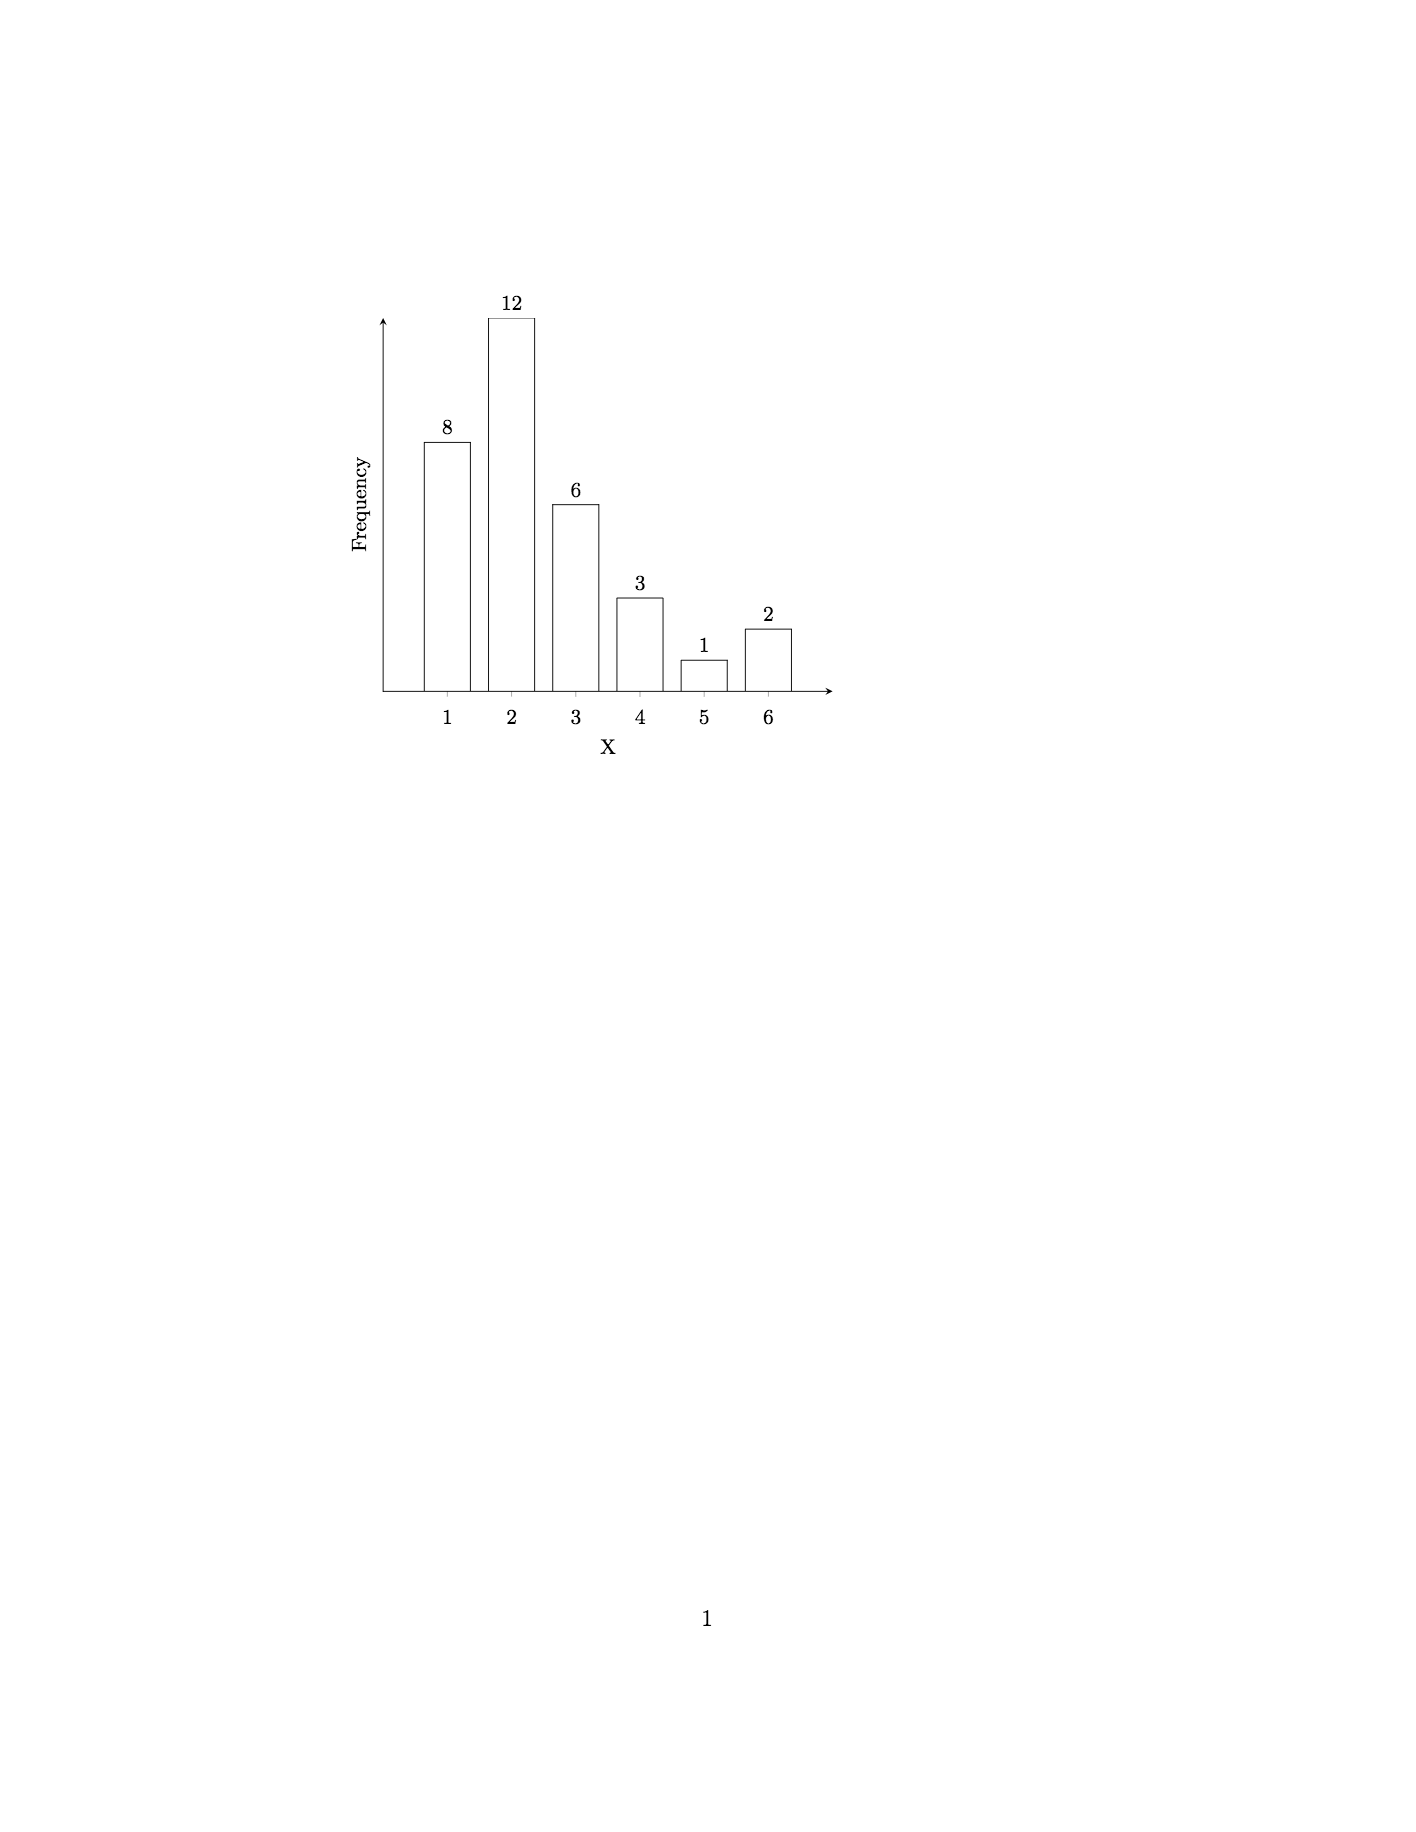
\includegraphics[width=1\linewidth]{images/frequencyhistogram.png}

		
		
%
\par
Experiment with creating your own histogram by inputting your data into the interactive cell below.
\begin{lstlisting}[style=sageinput]
#  This function is used to convert an input string into separate entries
def g(s): return str(s).replace(',',' ').replace('(',' ').replace(')',' ').split()

@interact
def _(freq = input_box("1,1,1,1,2,2,2,3,3,3,3,1,5",label="Enter data separated by commas")):
    freq = g(freq)
    freq = [int(k) for k in freq]
    m = min(freq)
    M = max(freq)
    bn = M-m+1
    histogram( freq, range=[m-1/2,M+1/2], bins = bn, align="mid", linewidth=2, edgecolor="blue", color="yellow").show()
\end{lstlisting}


		%
\par
Relative Frequency Histograms - In this case, area describes your data.  Notice in the interactive cell above that each bar is of width one. Therefore, frequency = area. In some instances where data may be grouped the total width of the interval may be different and so the height will need to be adjusted so that the total area of each bar corresponds to the relative frequency of that category.%
\par
Cummulative Histograms.  In these a running total is presented using all values from the given point and below.
\begin{lstlisting}[style=sageinput]
#  This function is used to convert an input string into separate entries
def g(s): return str(s).replace(',',' ').replace('(',' ').replace(')',' ').split()

@interact
def _(freq = input_box("1,1,1,1,2,2,2,3,3,3,3,1,5",label="Enter data separated by commas")):
    freq = g(freq)
    freq = [int(k) for k in freq]
    top = len(freq)
    m = min(freq)
    M = max(freq)
    bn = M-m+1
    histogram( freq, range=[m-1/2,M+1/2], cumulative = "true", bins = bn, align="mid", linewidth=2, edgecolor="blue", color="yellow").show(ymax=top)
\end{lstlisting}
		
%
\typeout{************************************************}
\typeout{Subsection 1.8.2 Stem-and-Leaf Plot}
\typeout{************************************************}
\subsection[{Stem-and-Leaf Plot}]{Stem-and-Leaf Plot}\label{subsection-4}
 - Histogram with data. Using the state population data above, consider organizing the data but using a "two-pass sort" where you first roughly break data up into groups based upon ranges which relate to their first digit(s). In this case, let's break up into groups according to populations corresponding to 0-4 million, 5-9 million, 10-14 million, 15-19, million, 20-24 million, 25-29 million, 30-35 million, and 35-39 million. We can represent these classes by using the stems 0L, 0H, 1L, 1H, 2L, 2H, 3L, and 3H where the L and H represent the one's digits L in {0, 1, 2, 3, 4} and H in {5, 6, 7, 8, 9}.  Once we group the data into these smaller groups then we can write the remaining portion of the number horizontally as leaves (in this case with one decimal place for all values.) This gives a step-and-leaf plot. If we additionally sort the data in the leaves then this gives you an ordered stem-and-leaf plot. For the state population data, the ordered stem-and-leaf plot is given by
		
	
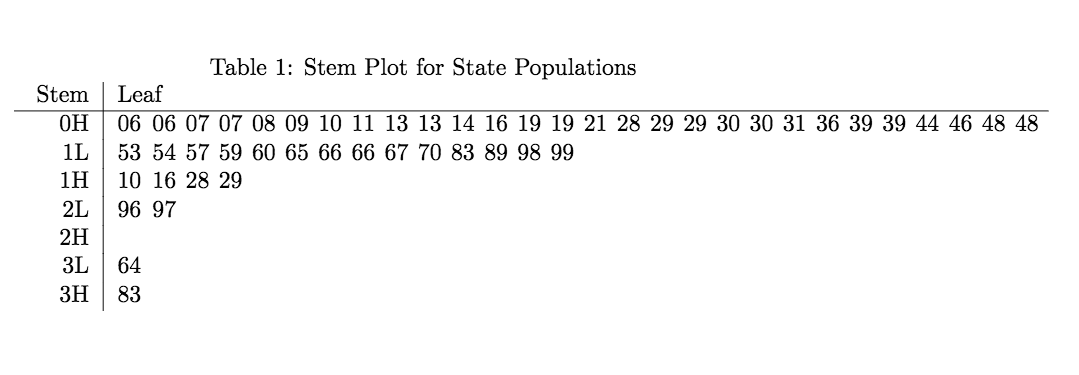
\includegraphics[width=1\linewidth]{images/stemandleaf.png}


Notice how it is easy to now see that most state populations are relatively small and that there are relatively few states with larger population. Also, notice that you can use this plot to relatively easily identify minimum, maximum, and other order statistics.		
%
\typeout{************************************************}
\typeout{Subsection 1.8.3 Box and Whisker Diagram (Box Plot)}
\typeout{************************************************}
\subsection[{Box and Whisker Diagram (Box Plot)}]{Box and Whisker Diagram (Box Plot)}\label{subsection-5}
This graphical display identifies the "5-number-summary" associated with the minimum, quartiles, and the maximum. That is, \(y_1, Q_1, Q_2, Q_3, y_n\).  These values separate the data roughly into quarters. To distinguish these quarters connect \(y_1\) and \(Q_1\) with a straight line (a whisker) and do the same with \(Q_3\) and \(y_n\). Use a box to connect \(Q_1\) with \(Q_2\) and the same to connect \(Q_2\) with \(Q_3\). Then the boxed areas also identify the IQR.  
%
\begin{lstlisting}[style=sageinput]
data <- c (0.6,0.6,0.6,0.7,0.7,0.8,0.9,1,1.1,1.3,1.3,1.4,1.6,1.9,1.9,2.1,2.8,2.9,2.9,3,3,3.1,3.6,3.9,3.9,4.4,4.6,4.8,4.8,5.3,5.4,5.7,5.9,6,6.5,6.6,6.6,6.7,7,8.3,8.9,9.8,9.9,10,11.6,12.8,12.9,19.6,19.7,26.4,38.3)
paste("Inter Quantile Range =",IQR(data))
paste("Box and Whisker Diagram - Box Plot):")
boxplot(data, horizontal=TRUE)
\end{lstlisting}
\par

You can produce something similar using Sage. Notice the different way that it is presented but the ideas are the same. For this one, once you evaluate the cell, you will need to click on "boxplot.png" to open up the actual box plot image as a file.
%
\begin{lstlisting}[style=sageinput]
from pylab import boxplot,savefig,close
@interact
def _(data = input_box([0.6,0.6,0.6,0.7,0.7,0.8,0.9,1,1.1,1.3,1.3,1.4,1.6,1.9,1.9,2.1,2.8,2.9,2.9,3,3,3.1,3.6,3.9,3.9,4.4,4.6,4.8,4.8,5.3,5.4,5.7,5.9,6,6.5,6.6,6.6,6.7,7,8.3,8.9,9.8,9.9,10,11.6,12.8,12.9,19.6,19.7,26.4,38.3],label="Enter Your Data:")):
    B = boxplot(data, notch=True, sym='x', vert=False)
    savefig("boxplot.png")
    close()
\end{lstlisting}
\typeout{************************************************}
\typeout{Subsection 1.8.4 Density Plots}
\typeout{************************************************}
\subsection[{Density Plots}]{Density Plots}\label{subsection-6}

A Density Plot can be created to visually interpret if the variable is close to normal
%
\begin{lstlisting}[style=sageinput]
library(e1071)
par(mfrow=c(1,2))    # graph into two columns
plot(density(cars$speed), main="Density Plot: Speed", ylab="Frequency", sub=paste("Skewness:", round(e1071::skewness(cars$speed),2)))
\end{lstlisting}
\par

www.machinelearningplus.com
%
\typeout{************************************************}
\typeout{Section 1.9 Exercises}
\typeout{************************************************}
\section[{Exercises}]{Exercises}\label{section-9}
Complete the online WebWorK homework set "Computational Measures".%
\begin{exercise}\label{exercise-3}
Create a data set with about 10 elements. For your data set, compute each of the measures from this chapter and present your data using a frequency histogram.%
\end{exercise}
\begin{exercise}\label{exercise-4}
Find a "real-world" data set (similar perhaps to the Census data presented above.) Compute each of the measures from this chapter. Interpret and present your conclusions in an electronic report which can include an excel spreadsheet.%
\end{exercise}
\typeout{************************************************}
\typeout{Chapter 2 Regression}
\typeout{************************************************}
\chapter[{Regression}]{Regression}\label{CurveEstimation}
\typeout{************************************************}
\typeout{Section 2.1 Introduction}
\typeout{************************************************}
\section[{Introduction}]{Introduction}\label{section-10}

Given a set of data points \((x_0,y_0), (x_1,y_1), ... (x_n,y_n)\), it is often desirable to have a nice continuous formula \(y = f(x)\) that expresses the general nature of those data points. Such a formula "interpolates" the data points if \(y_k = f(x_k)\), that is the formula gives a graph that exactly passes through each of the given data points.%
\par

On the other hand, sometimes the data points are known to be only approximate or the complexity of the formula needed to interpolate all of the data points exactly is too large. In this case, the formula may only be required to return values that are relatively close to the data points. Such a formula is said to "approximate" and gives \(y_k \approx f(x_k)\). Below, we consider ways to create useful models that approximate the data points.
%
\par

From basic algebra, if you are given two distinct points then there is one line which passes exactly through (i.e. interpolates) both. There are many ways to create this linear model but for points \((x_0,y_0), (x_1,y_1)\),

\begin{equation*} y = \frac{y_1 - y_0}{x_1 - x_0}(x - x_0) + y_0\end{equation*}

is the linear function which passes through both points if the x-values are distinct.  If the x's are equal then 
\begin{equation*} x = x_0\end{equation*}
is linear and interpolates both data points. 
However, once you collect three or more points it is likely that there is no line which exactly "interpolates" all of the points. So, if we desire a linear model then we must settle for a model that approximates. In this chapter, you will investigate how to create polynomial functions which in some manner approximate a collection of data point in some "best" manner.
%
\begin{exercise}\label{exercise-5}
\end{exercise}
\typeout{************************************************}
\typeout{Section 2.2 Linear Regression}
\typeout{************************************************}
\section[{Linear Regression}]{Linear Regression}\label{section-11}

In this section, we will presume only one independent variable x and one dependent variable y.
%
\par

Consider a collection of data points 
\begin{equation*}(x_0,y_0), (x_1,y_1), ... , (x_n,y_n)\end{equation*}
and a general linear function 
\begin{equation*}f(x) = mx + b.\end{equation*}
It is possible but generally unlikely that each of the given data points are exactly interpolated by the linear function. However, you may notice that the data points exhibit a linear tendency or that the underlying physics might suggest a linear model. If so, you may find it easier to predict values of y for given values of x using a linear approximation. Here you will investigate a method for doing so called "linear regression", "least-squares", or "best-fit line". 
%
\par

But why even bother creating a formula (a line here) to approximate data that does not satisfy that formula? Remember that you would expect collected data to vary slightly as one repeatedly collects that data in the same way that you would expect to make a slightly different score on repeated attempts at exams on the same material. Creating a formula that is close to your data gives a well-defined way to predict a y value for a given x value. This predictive behavior is illustrated in the exercise below.
%
\begin{exercise}[{WebWork}]\label{exercise-6}

		Consider using the following best-fit line for approximation.
		%
\par\medskip
